\documentclass{article}
\usepackage{amsmath}
\usepackage{graphicx}

\title{Stereoselective Addition of Tertiary Carbon Radicals}
\author{Eric Ma, Thinh Nguyen, Manny Teutla}
\date{Chem 250L}

\begin{document}

\maketitle

\textbf{Assignment 6.1}
Limitations of transition state theory
\begin{enumerate}
	\item Is the activated complex equivalent to the "dividing surface" ? \\
	Assuming $k_2 >> 0$, the reaction should not proceed in the reverse direction from the transition state to the product.
	Therefore, the activated complex is equivalent to the "dividing surface".

	\item Give an example of a chemical reaction where TST fails, and explain why. \\
	Transition state theory relies on transition states existing long enough for a Boltzman distribution to form.
	In multistep reactions, there are multiple transition step before the product is produced, so each step would need to reach quasi-equilibrium in before being able to proceed.
	TST fails when any step's intermediate structure is too short lived.
\end{enumerate}

\textbf{Assignment 6.2}
Eyring equation

\begin{enumerate}
	\item Derive an expression for $k_1$ in terms of the change in Gibbs free energy of activation, $\Delta G^\ddag$, for the quasi-equilibrium reaction in Eq. 6.1.
	\begin{equation*}
	\begin{split}
		\Delta G^\ddag & = - R T ln[ K^\ddag ] \\ 
		& = - R T ln[ \frac{h}{k_B T} k_1 ] \\
		ln[ \frac{h}{k_B T} k_1 ] & = - \frac{\Delta G^\ddag}{R T} \\
		k_1 ( \frac{h}{k_B T} ) & = \text{Exp}[ - \frac{\Delta G^\ddag}{R T} ] \\
		k_1 & = \frac{k_B T}{h} \text{Exp}[ - \frac{\Delta G^\ddag}{R T} ] 
	\end{split}
	\end{equation*}

	\item Consider two competing reactions of the same passing through two different transition states.
	Derive an expression for the relative yield of the two resulting products in terms of the difference in Gibbs free energies of activation, sometimes called $\Delta \Delta G^\ddag$, under the assumption of kinetic control.
	\begin{equation*}
	\begin{split}
		\frac{k_1}{k_2} & = \frac{\text{Exp}[ - \frac{\Delta G_1^\ddag}{R T} ]}{\text{Exp}[ - \frac{\Delta G_2^\ddag}{R T} ]} \\
		& = \text{Exp}[ \frac{\Delta G_2^\ddag - \Delta G_1^\ddag}{R T} ] \\
		& = \text{Exp}[ \frac{\Delta \Delta G^\ddag}{R T} ]  
	\end{split}
	\end{equation*}
\end{enumerate}

\textbf{Assignment 6.3}
Lewis structures and their limitations
% Fix graphics to better represent the structure's sp$^3$ hybridization
\begin{enumerate}
	\item Draw the Lewis structure of the reacting radical for the reaction in Fig. 6.2.2.
		\begin{figure}[h]
			\centering
			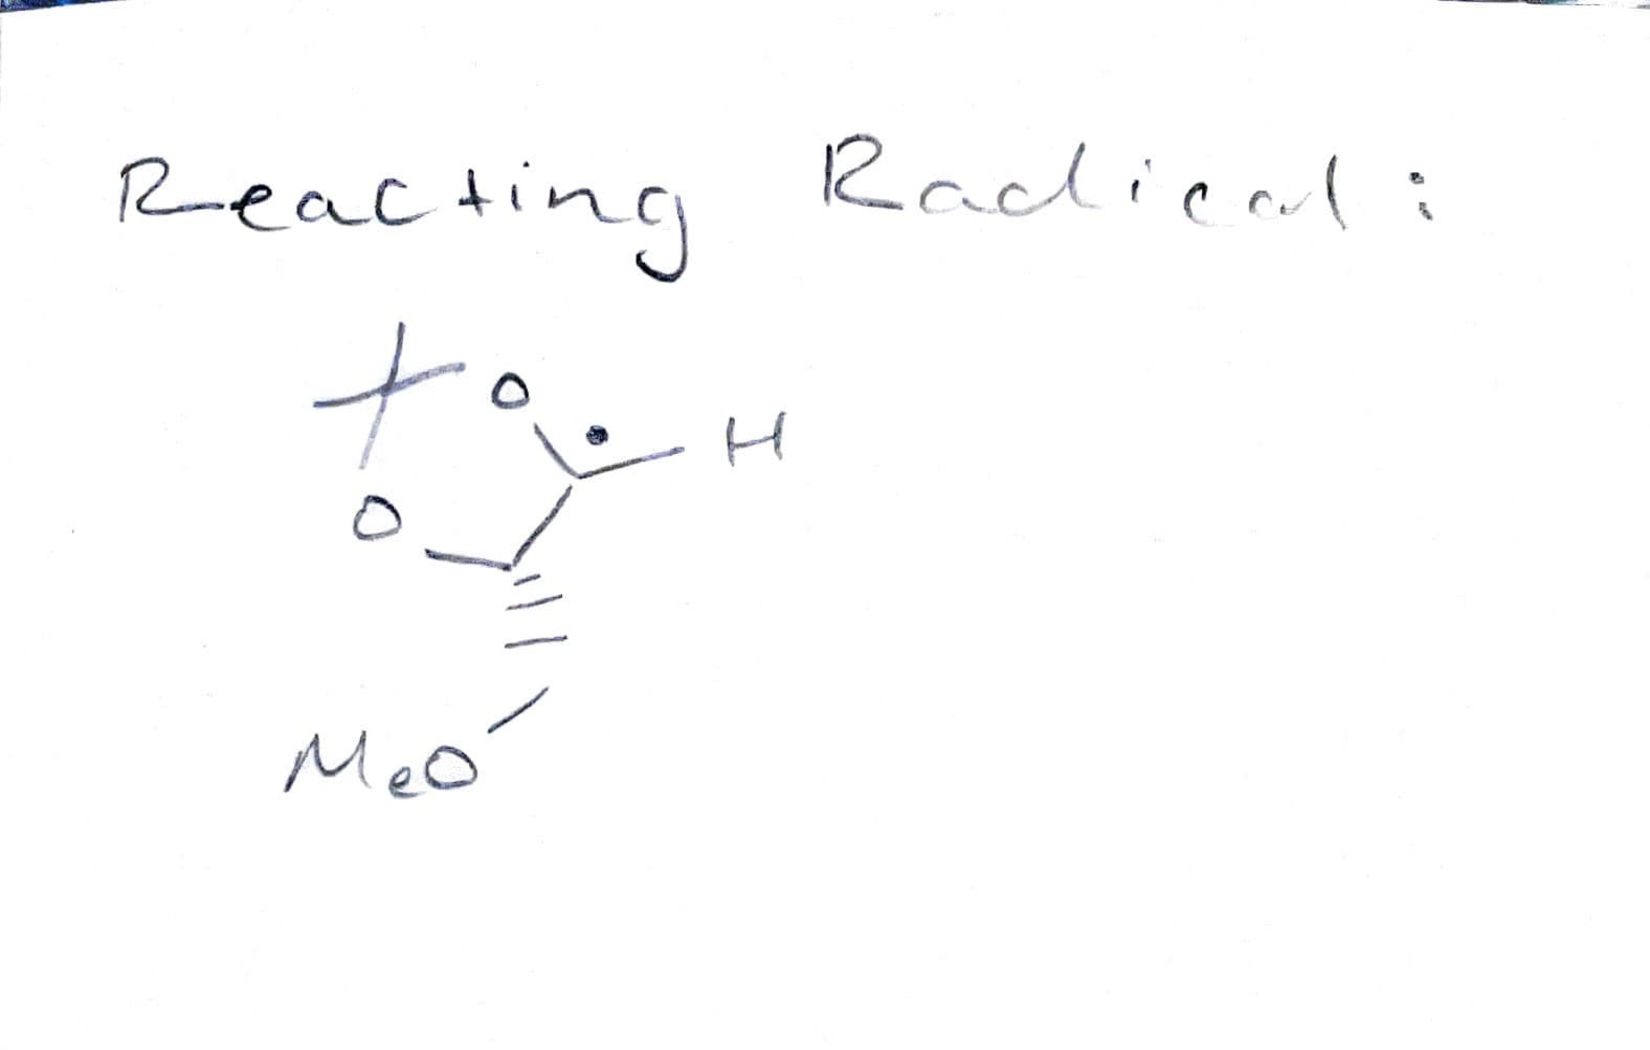
\includegraphics[width=\textwidth]{images/reacting-radical.pdf}
		\end{figure}
\newpage
	\item Draw structures for the transition states leading to the syn and the anti products.
		\begin{figure}[h]
			\centering
			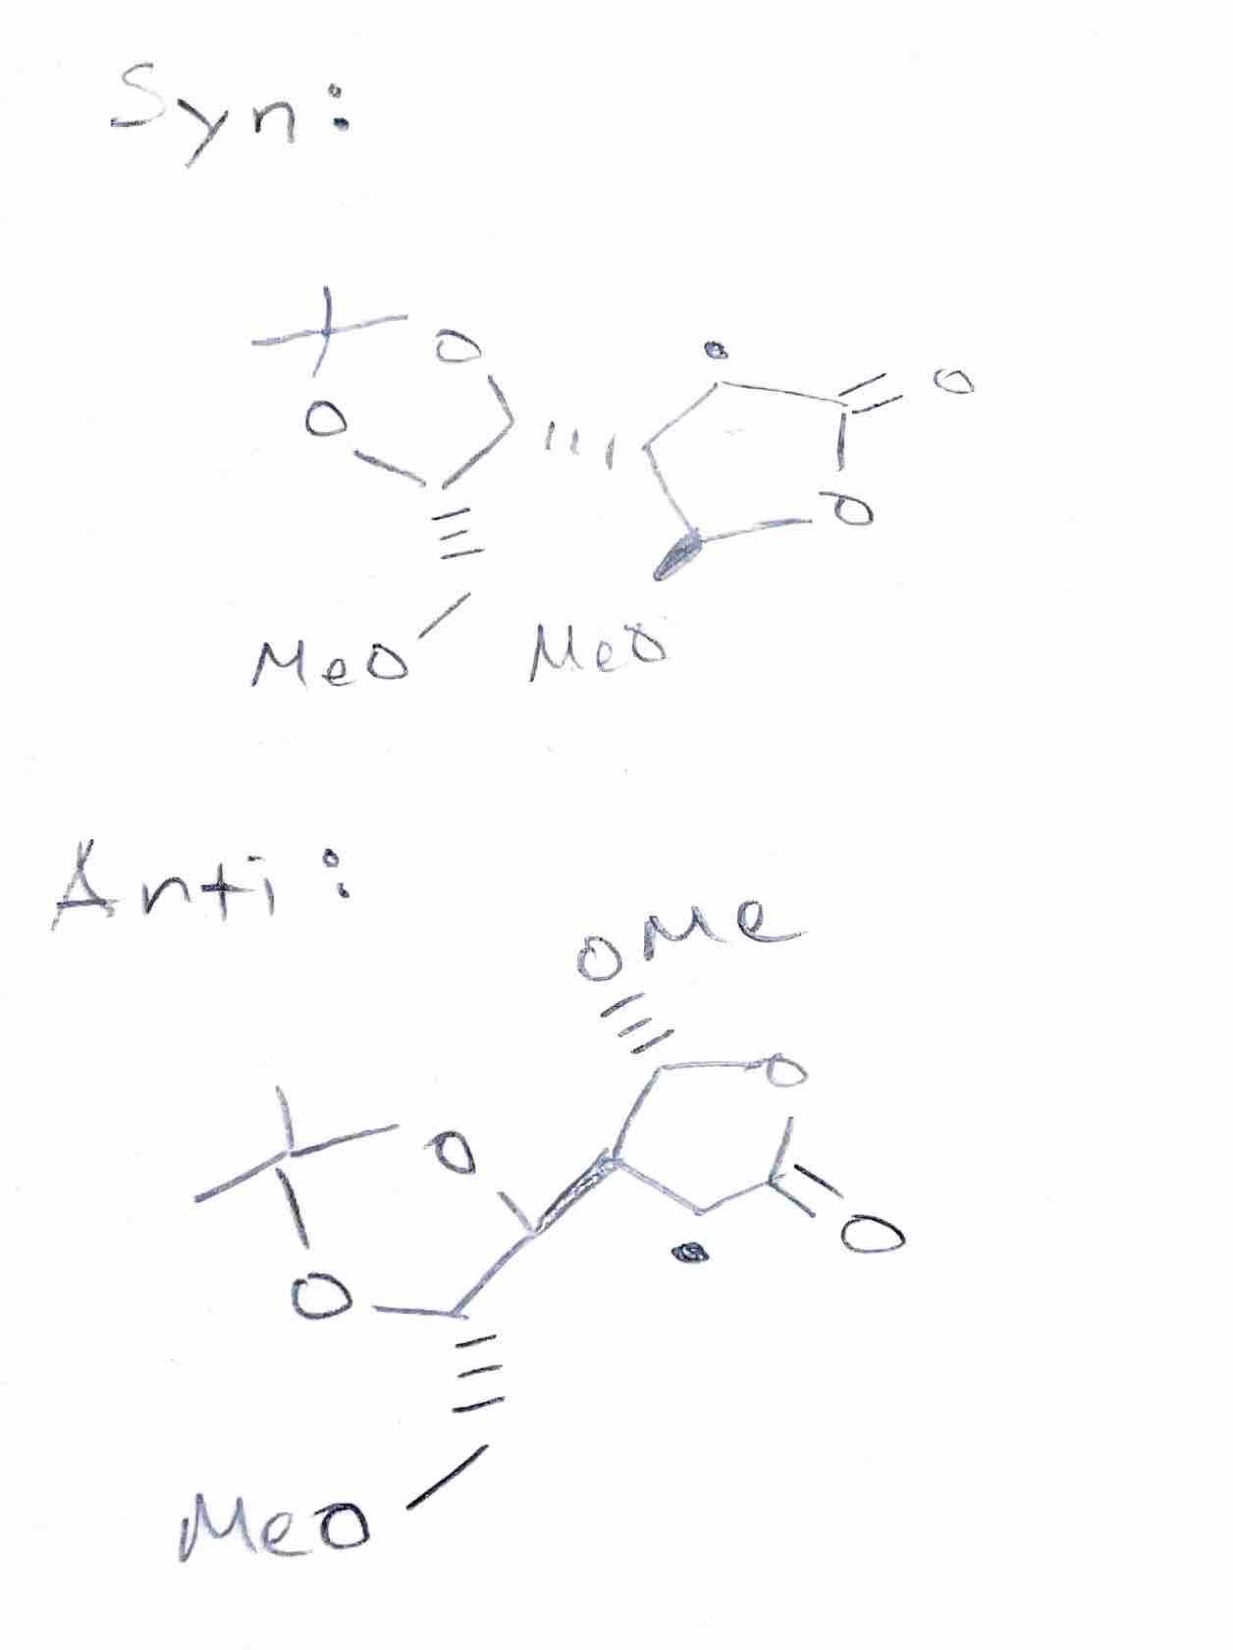
\includegraphics[width=0.9\textwidth]{images/syn-anti.pdf}
		\end{figure}

	\item Why is the syn/anti selectivity difficult to predict without a calculation ? \\
	The carbon radical stereocenter is sp$^3$ hybridized, so simple factors like steric hinderences are less obvious in determining selectivity.
	
\end{enumerate}

\enddocument
